\chapter{Conclusion}
\label{Conclusion}

The aim of this thesis was to continue the theoretical work of Romain Chanal and finish the first phase of the development process of the Artificial Eye. This included building, qualifying and optimising the optical measurement system. Figure \ref{ChainConclusion} gives an overview of the development process of the Artificial Eye, with the steps performed during this thesis green-bordered.

\begin{figure}[h]
\begin{center}
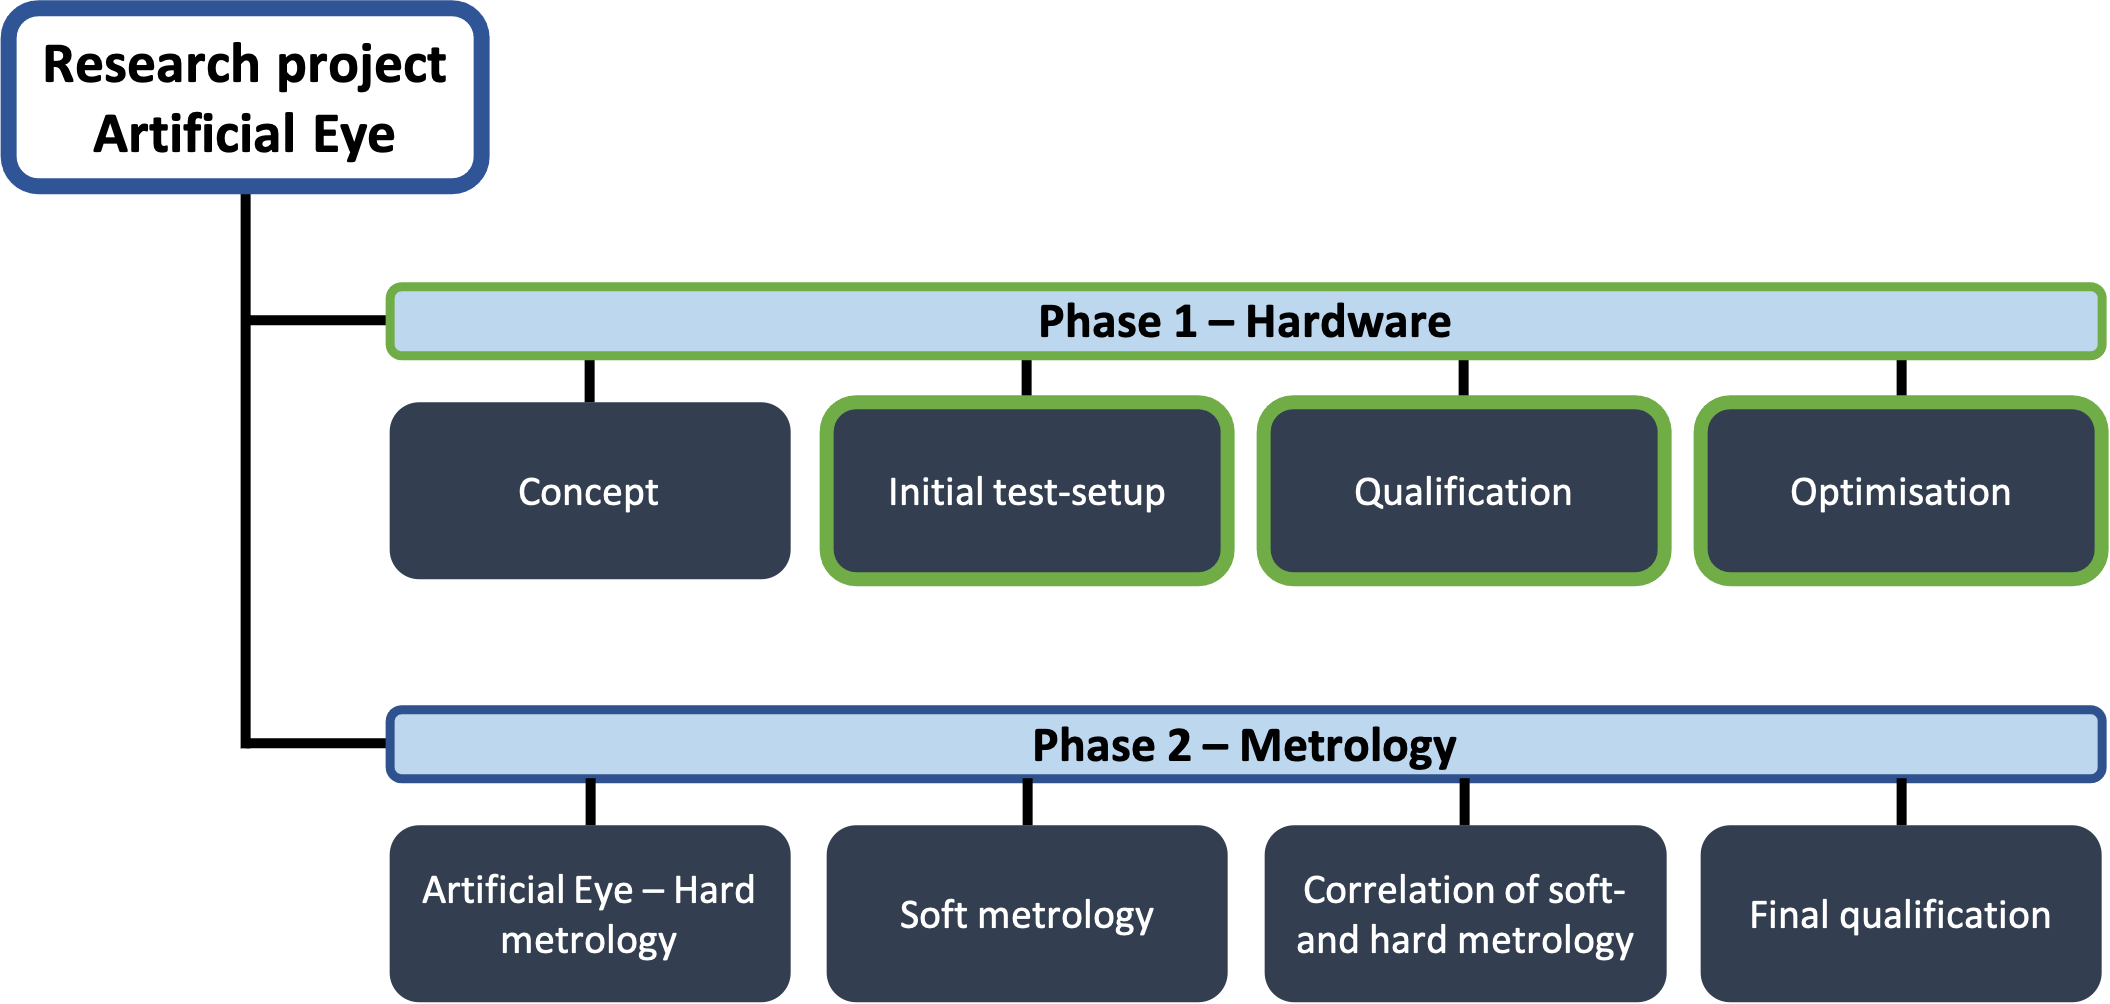
\includegraphics[width=12cm]{Pictures/ChainConclusion}
\caption[Overview of the development made during this thesis]{Overview of the development made during this thesis: Green - Completed}
\label{ChainConclusion}
\end{center}
\end{figure}

The first part, the building of the test setup, consisted of different steps. First, all the necessary parts of the optical setup of the Artificial Eye were ordered and assembled. Next, the needed power and data connections were made, in order to communicate with the system. Finally, to run the system, a software was developed featuring easy to use graphical user interface.\\

The process of the qualification of the initial test setup, was split in three different tests and their evaluation. They were designed to strategically test the capability of the optical system regarding the ability to transmit light, the common focus of the camera system as well as the maximum resolution of the system.\\

The last step in development phase one of the Artificial Eye, was the optimisation of the system. These optimisations were dependant on the results of the test conducted during step 2. The first test was about the light transmission capabilities of the system. Its evaluation showed that, caused by the design of the optical system, the four cameras and especially the three monochromatic cameras were not receiving enough light. This conclusion caused a major redesign of the colour filters used in the system as well as the decision to use a different lens in order to pick up more light.\\

The aim of the focus test was to ensure that all four cameras of the system are sharing the same focal plane. The evaluation showed that one of the cameras did not meet this requirement. This problem was solved by rearranging the optical system. This rearrangement also had impact onto the light transmission capabilities of the system, which were slightly decreased. 

The aim of the last test was to investigate the maximum resolution of the Artificial Eye. It was essential that the optical system had a better resolution than the human eye in order to acquire usable data. The evaluation showed that the Artificial Eye fulfils this requirement. Therefore no additional changes needed to be made to the system.\\

With the made changes the first phase of the development process of the research project Artificial Eye was completed. The system is now able to acquire data reliably in an automated way. Further it can be controlled easily via an graphical user interface and meets all requirements in order to continue with the second phase in the development process.\\


\section{Personal conclusion}

Generally and personally speaking, because it took a long time to get into the project, the beginning of this thesis was very challenging. A lot of knowledge about optics was needed in order to understand the complex working principle of the Artificial Eye. The complexity of the research project and the tasks it is trying to achieve, lead to changes made during this thesis. Each change required a lot of theoretical research to get the knowledge about how it would impact the functionality of the system.\\

While preparing, executing and evaluating the different tests it was possible to earn a lot of practical and theoretical experience in different topics. In addition to that, it was very interesting, to work together with many people having different backgrounds and professions. This allowed to get an insight into a variety of research topics, such as optics, surface metrology and industrial design.\\

In my point of view, this bachelor thesis and my time in Sweden, gained many new experiences and knowledge. It not only fulfilled all my personal expectations but exceeded them.




